\begin{frame}
    \begin{centering}
        \vskip5ex plus 1filll
        {\usebeamerfont{title page title}\usebeamercolor[fg]{title page} Nodal Analysis\\[1.5ex]}
        \vskip0pt plus 1filll
    \end{centering}
\end{frame}

\begin{frame}{Example Circuit: Tone Stage}
    \begin{figure}
        \centering
        \begin{circuitikz}[node distance=0.5cm] \draw[color=white]
            (0, 0) node[op amp] (opamp) {}
            (opamp.+) to[short, l_=+4.5V,-o] (-1.2, -1.0)
            (opamp.-) to[R, l_=R22] (-3, 0.5)
            to[short, l=Vin,-o] (-3.5, 0.5)
            (-3, 0.5) to[R, l=R21] (-3, 2.0)
            (-3, 4.5) -- (-3, 4.0) to[american potentiometer, l_=RV2, n=mypot] (-3, 2.0)
            (mypot.wiper) to[C, l=C14] (-1.2, 3.0)
            (opamp.-) -- (-1.2, 3.0)
            to[R, l=R24] (1.5, 3.0)
            (-3, 4.5) to[R, l=R23] (1.5, 4.5)
            -- (1.5, 0.0)
            (opamp.out) -- (1.5, 0.0) to[short, l_=Vout,-o] (2.5, 0.0)
          ;
        \end{circuitikz}
        \caption{\label{fig:ToneControl}{\it Klon Centaur Tone Control Circuit}}
    \end{figure}
\end{frame}

\begin{frame}{Nodal Analysis: Continuous Time}
    1. Convert the circuit to the Laplace Domain,
    using the Laplace variable $s = j\omega$. The
    complex impedance of each principal circuit component
    is defined as:
    \begin{equation}
        Z_R = R, \quad Z_C = \frac{1}{Cs}, \quad Z_L = Ls
    \end{equation}
\end{frame}

\begin{frame}{Nodal Analysis: Continuous Time}
    2. Form the Laplace domain transfer function.\footcite{Maby}
    \begin{equation}
        \frac{V_{out}(s)}{V_{in}(s)} = {\scriptscriptstyle \frac{C_{14}\left(\frac{1}{R_{22}} + \frac{1}{R_{21} + R_{v2b}}\right)s
        + \frac{1}{R_{22}}\left(\frac{1}{R_{21} + R_{v2b}} + \frac{1}{R_{23} + R_{v2a}}\right)}{
          C_{14}\left(\frac{1}{R_{23} + R_{v2a}} + \frac{1}{R_{24}}\right)s
        + \frac{-1}{R_{24}}\left(\frac{1}{R_{21} + R_{v2b}} + \frac{1}{R_{23} + R_{v2a}}\right)}}
    \end{equation}
\end{frame}

\begin{frame}{Nodal Analysis: Discrete Time}
    3. Use a conformal map to map from the s-plane to z-plane
    (often the bilinear transform).\footcite{pasp}
    \begin{equation}
        s \leftarrow \frac{2}{T} \frac{1 - z^{-1}}{1 + z^{-1}}
    \end{equation}
\end{frame}

\begin{frame}{Nodal Analysis: Discrete Time}
    4. Implement the system as a digital filter.
    \begin{equation}
        y[n] = b_0 x[n] + b_1 x[n-1] + b_2 x[n-2] - a_1 y[n-1] - a_2 y[n-2]
    \end{equation}
    \vspace{-0.5cm}
    \begin{figure}
        \centering
        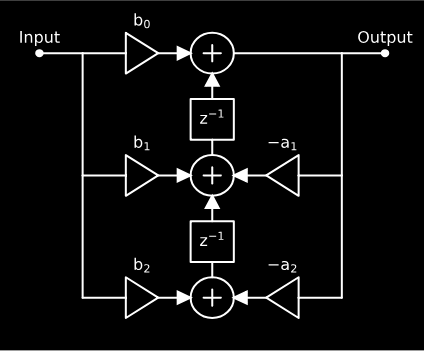
\includegraphics[height=2.25in]{Figures/TDF-II.png}
    \end{figure}
\end{frame}

\begin{frame}{Discretization Considerations}
    \vspace{1ex}
    \begin{itemize}
        \itemsep0em
        \item Frequency warping
        \item Stability
    \end{itemize}
    \begin{figure}
        \centering
        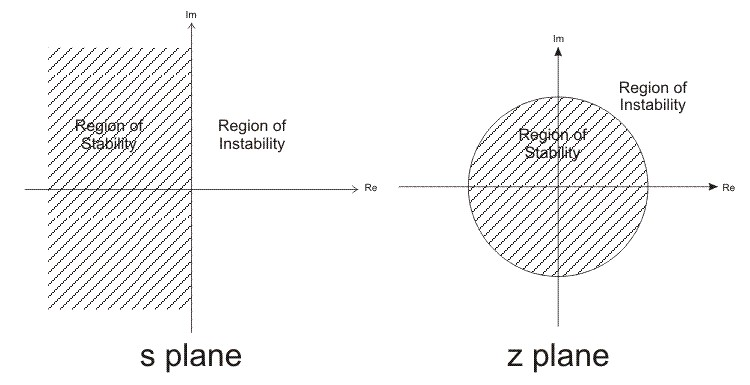
\includegraphics[height=2.0in]{Figures/bilinear_mapping.jpg}
    \end{figure}
\end{frame}

\begin{frame}{Tone Stage Frequency Response}
    \begin{figure}
        \centering
        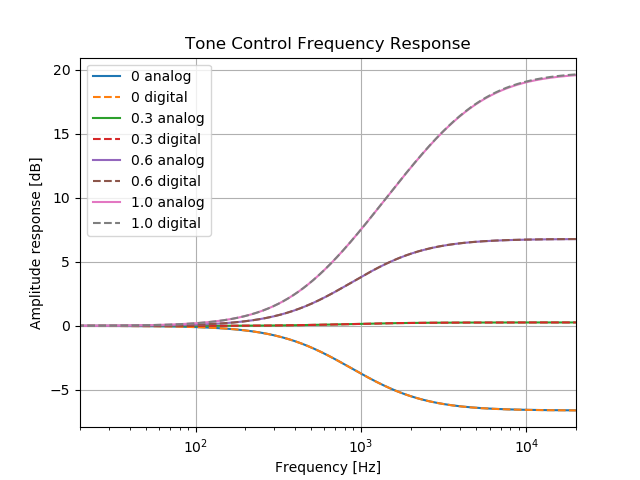
\includegraphics[height=2.75in]{../Paper/Figures/ToneFreq.png}
    \end{figure}
\end{frame}

\begin{frame}{Nodal Analysis}
    \begin{columns}
        \begin{column}{0.5\linewidth}
            \hspace{-1ex}
            Advantages:
            \vspace{1ex}
            \begin{itemize}
                \itemsep0.5em
                \item Simple and computationally efficient circuit models
                % \item Requires a fairly minimal understanding of circuit theory and DSP
            \end{itemize}
        \end{column}
        \begin{column}{0.5\linewidth}
            \hspace{-1ex}
            Disadvantages:
            \vspace{1ex}
            \begin{itemize}
                \itemsep0.5em
                \item Cannot be used to model nonlinear circuits (can be extended with Modified Nodal Analysis)
                \item Sometimes difficult to compute parameter changes
            \end{itemize}
        \end{column}
    \end{columns}
\end{frame}
